\documentclass[aspectratio=169]{beamer} % 16:9 aspect ratio to match modern screens
\usefonttheme{serif}

% --- Packages ---
\usepackage[T1]{fontenc}
\usepackage[utf8]{inputenc}

\usepackage{lmodern}

\usepackage{dsfont}
\usepackage[dvipsnames]{xcolor}
\usepackage{tcolorbox}
\tcbuselibrary{skins, theorems}
\usepackage{multimedia} % Included for video support
\usepackage{fontawesome5}
\usepackage[normalem]{ulem} % The normalem option keeps your \emph{} styling normal
\usepackage{cancel}
\usepackage{amsmath}
\usepackage{mathtools}
\usepackage{circuitikz}
\usepackage{pgfplots}
\pgfplotsset{compat=1.18}
\usepackage{pgfplotstable}
\usetikzlibrary{arrows.meta}
\usepackage{tkz-tab}
\usepackage{tikz}
\usepackage{tikz-cd}
\tikzstyle{lien}
=[->,>=stealth,rounded
corners=5pt,thick]
\tikzset{
	invisible/.style={opacity=0, text opacity=0},
	visible on/.style={alt={#1{}{invisible}}},
	alt/.code args={<#1>#2#3}{%
		\alt<#1>{\pgfkeysalso{#2}}{\pgfkeysalso{#3}}%
	},
}
\usepackage{amssymb}
\usetikzlibrary{arrows.meta, positioning, calc}
\usepackage{esvect}
\usepackage{graphicx}
\usepackage{wasysym}
\usepackage{qrcode}

\DeclareMathAlphabet{\mathpzc}{OT1}{pzc}{m}{it}

% --- Bibliography ---
\usepackage[
backend=bibtex,
giveninits=true,
style=numeric,
maxbibnames=99,
mincitenames=1,
maxcitenames=4
]{biblatex}
\addbibresource{bibi.bib}
\setbeamerfont{footnote}{size=\tiny}
\setbeamercolor{footnote mark}{fg=brandAccent}

% --- Color Definitions (from theme.scss) ---
\definecolor{brandAccent}{HTML}{D77E62}
\definecolor{brandPurple}{HTML}{7201A8}
\definecolor{brandAccentDark}{HTML}{B7654B}
% Approximating the transparent #e6a08a4a background
\colorlet{brandAccentLight}{brandAccent!5!white}

\colorlet{brandRed}{brandAccent!20!red}

% --- Beamer Color & Font Settings ---
\setbeamercolor{title}{fg=brandAccent}
\setbeamercolor{frametitle}{fg=brandAccent}
\setbeamercolor{structure}{fg=brandAccent} % Colors bullets and standard structural elements
\setbeamercolor{author}{fg=black}
\setbeamercolor{date}{fg=black}

% --- Link & Reference Styling ---
\renewcommand{\eqref}[1]{\hyperref[#1]{\color{brandAccent}(\ref*{#1})}}
\hypersetup{
	colorlinks=true,
	linkcolor=brandAccent,
	urlcolor=brandAccent,
	citecolor=brandAccent
}

% Clean up the presentation (removes navigation symbols)
\setbeamertemplate{navigation symbols}{}
\setbeamertemplate{footline}[page number]

% --- Custom Theorem Block (Replicating the CSS Bubble Style) ---
\newtcbtheorem{mythm}{Theorem}{
	enhanced,
	colback=brandAccentLight,
	colframe=brandAccent,
	boxrule=1pt,
	arc=4mm,          % 14px border radius
	auto outer arc,
	coltitle=white,
	colbacktitle=brandAccent,
	fonttitle=\bfseries\small,
	top=5mm,  % <--- INCREASES VERTICAL SPACE BETWEEN BUBBLE AND TEXT
	bottom=2mm, % Optional: gives a little breathing room at the bottom too
	% Pill-shaped floating title
	separator sign={},
	title style={borderline={0pt}{0pt}{brandAccent}, rounded corners, arc=2mm},
	attach boxed title to top left={xshift=4mm, yshift=-3mm},
	boxed title style={
		size=small,
		top=-0.5mm,    % <--- Shrink top padding
		bottom=-0.5mm, % <--- Shrink bottom padding
		left=1mm,     % <--- Shrink left padding
		right=1mm     % <--- Shrink right padding
	}
}{thm}
\newtcbtheorem{myprop}{Proposition}{
	enhanced,
	colback=brandAccentLight,
	colframe=brandAccent,
	boxrule=1pt,
	arc=4mm,          % 14px border radius
	auto outer arc,
	coltitle=white,
	colbacktitle=brandAccent,
	fonttitle=\bfseries\small,
	top=3mm,
	bottom=2mm,
	separator sign={},
	% Pill-shaped floating title
	title style={borderline={0pt}{0pt}{brandAccent}, rounded corners, arc=2mm},
	attach boxed title to top left={xshift=4mm, yshift=-3mm},
	boxed title style={
		size=small,
		top=-0.5mm,    % <--- Shrink top padding
		bottom=-0.5mm, % <--- Shrink bottom padding
		left=1mm,     % <--- Shrink left padding
		right=1mm     % <--- Shrink right padding
	}
}{prop}

% --- Maths ---
\def\argmin#1{{\underset{#1}{\mathrm{arg}\,\mathrm{min}\ }}}
\def\argmax#1{{\underset{#1}{\mathrm{arg}\,\mathrm{max}\ }}}
\def\d{\mathrm{d}}
\def\R{\mathbb{R}}
\newcommand{\cev}[1]{\reflectbox{$\vec{\reflectbox{$#1$}}$}}
\newcommand{\rust}[1]{\textcolor{brandAccent}{#1}}
\newcommand{\purp}[1]{\textcolor{brandPurple}{#1}}
\renewcommand{\exp}[1]{\mathrm{exp}\left(#1\right)}
\renewcommand{\ln}[1]{\mathrm{ln}\left(#1\right)}
\newcommand{\myatop}[2]{%  % a macro with LaTeX-style syntax
	\fontdimen10\textfont2=\fontdimen9\textfont2% using wipet's suggestion
	{\begingroup#1\endgroup\atop#2}}
\newcommand{\pN}{\mathpzc{N}}
\newcommand{\pn}{\mathpzc{n}}

% --- Title Information ---
\title{
	Iterating semi-discrete JKO steps by stochastic approximation
}
\author{Quentin Giton \\
	{\small Join work with Thomas Gallouët (LMO) and Ziad Kobeissi (L2S)}}
\institute{Laboratoire de Mathématiques d'Orsay}
\date{November 12th} % Leave empty if no date is desired

\setbeamertemplate{page number in head/foot}{\insertframenumber{} / \inserttotalframenumber}

\begin{document}
	\begin{frame}
		\titlepage
	\end{frame}
	
	\begin{frame}[t]{(Euclidean) Gradient flows}
		\begin{equation*}
			E\::\:\R^d\to\R,\qquad\dot x_t = -\nabla E(x_t)
		\end{equation*}
		
		\begin{itemize}
			\item \textbf{Explicit Euler:} $\tau>0$, $\nabla E(x_n^\tau)+\frac{x_{n+1}^\tau-x_n^\tau}{\tau}=0$.
			
			Needs $E$ to be differentiable.
			\vspace{\baselineskip}
			\item \textbf{Implicit Euler:} $\tau>0$, $\nabla E(x_{n+1}^\tau)+\frac{x_{n+1}^\tau-x_n^\tau}{\tau}=0$
			\vspace{\baselineskip}
			\item Equivalent to the variational problem
			\begin{equation*}
				x_{n+1}^\tau = \argmin{x\in\R^d} E(x)+\frac{1}{2\tau}\|x-x_n^\tau\|^2
			\end{equation*}
			Only needs a distance on $\R^d$!
			
		\end{itemize}
	\end{frame}
	
	\begin{frame}[t]{(Wasserstein) Gradient flows}
		We define recursively, starting from $\mu\in\mathcal{P}_2(\R^d)$
		\begin{equation*}
			\rho_0^\tau = \mu,\qquad \rho_{n+1}^\tau = \argmin{\rho\in\mathcal P_2(\R^d)} \mathcal E(\rho)+\frac{1}{2\tau}W_2(\rho,\rho_n^\tau)^2
		\end{equation*}
		
		\begin{itemize}[<+->]
			\item $W_2(\mu,\nu)$ is the optimal transport distance.
			\vspace{.5\baselineskip}
			\item Piecewise constant interpolation of the $(\rho_n^\tau)_n$ and letting $\tau\to0$ yields a curve in $\mathcal P_2(\R^d)$ solving (weakly) the continuity equation
			\begin{equation*}
				\partial_t\rho_t = -\mathrm{div}(\rho_t v_t)
			\end{equation*}
			for some vector field $v_t$ (related to $\mathcal E$).
			\vspace{.5\baselineskip}
			\item $\mathcal E(\rho)=\int V\rho+\int\rho\ln{\rho}$ yields the Fokker--Planck equation
			\begin{equation*}
				\partial_t\rho_t=\Delta\rho_t +\mathrm{div}(x\rho_t)
			\end{equation*}
		\end{itemize}
	\end{frame}
	
%	\begin{frame}[t]{Quick reminders on Optimal Transport 1/2}
%		\begin{center}
%			\resizebox{0.8\linewidth}{!}{
%				\begin{tikzpicture}[>=Stealth, scale=1.3]
%					\draw[->, thick] (-0.5, 0) -- (10.0, 0) node[right] {$\mathbb{R}$};
%					
%					\begin{scope}
%						\begin{scope}
%							\clip (0,0) 
%							.. controls (0.8, 0.1) and (1.2, 2.2) .. (2.0, 2.2)
%							.. controls (2.8, 2.2) and (3.2, 0.1) .. (4.0, 0) -- (4.0,0) -- (0,0) -- cycle;
%							\fill[brandAccent!30] (1.3, 0) rectangle (2.1, 2.5);
%						\end{scope}
%						
%						\draw[thick, brandAccent] (0,0) 
%						.. controls (0.8, 0.1) and (1.2, 2.2) .. (2.0, 2.2)
%						.. controls (2.8, 2.2) and (3.2, 0.1) .. (4.0, 0)
%						node[above=2pt] {$\mu$};
%						
%						\draw[brandAccent, thick, dashed] (1.3, 0) -- (1.3, 1.65);
%						\draw[brandAccent, thick, dashed] (2.1, 0) -- (2.1, 2.15);
%						\node[brandAccent!90!black] at (1.7, 0.8) {$\mu(A)$};
%						
%						\draw[brandAccent, line width=3pt] (1.3, 0) -- (2.1, 0);
%						\draw[brandAccent, thick] (1.3, -0.1) -- (1.3, 0.1); 
%						\draw[brandAccent, thick] (2.1, -0.1) -- (2.1, 0.1); 
%						\node[brandAccent!90!black, below=4pt] at (3.125, 0) {$A=\{x\in\mathbb{R}: T(x)\in B\}$};
%					\end{scope}
%					
%					\begin{scope}[xshift=5cm]
%						\begin{scope}
%							\clip (0,0) 
%							.. controls (1.0, 0.1) and (1.5, 1.4) .. (2.5, 1.4)
%							.. controls (3.5, 1.4) and (3.8, 0.1) .. (4.2, 0) -- (4.2,0) -- (0,0) -- cycle;
%							\fill[brandPurple!30] (1.6, 0) rectangle (3.2, 2.5);
%						\end{scope}
%						
%						\draw[thick, brandPurple] (0,0) 
%						.. controls (1.0, 0.1) and (1.5, 1.4) .. (2.5, 1.4)
%						.. controls (3.5, 1.4) and (3.8, 0.1) .. (4.2, 0)
%						node[above=2pt] {$\nu$};
%						
%						\draw[brandPurple, thick, dashed] (1.6, 0) -- (1.6, 1.025);
%						\draw[brandPurple, thick, dashed] (3.2, 0) -- (3.2, 1.15);
%						\node[brandPurple!90!black] at (2.4, 0.5) {$\nu(B)$};
%						
%						\draw[brandPurple, line width=3pt] (1.6, 0) -- (3.2, 0);
%						\draw[brandPurple, thick] (1.6, -0.1) -- (1.6, 0.1); 
%						\draw[brandPurple, thick] (3.2, -0.1) -- (3.2, 0.1); 
%						\node[brandPurple!90!black, below=4pt] at (2.4, 0) {$B$};
%					\end{scope}
%					
%					\draw[->, thick, black] (3.25, 1.5) to[bend left=30] node[above, text=black] {$T$} (6.25, 1.5);
%				\end{tikzpicture}
%			}
%		\end{center}
%		
%		% DYNAMIC TEXT BLOCK
%		\begin{itemize}%[<+->]
%			\item Given ground cost $c(\rust{x},\purp{y}) = \|\rust{x}-\purp{y}\|^2$
%			
%			\item Among all maps $T$ satisfying $\forall\textcolor{brandPurple}{B},\ \textcolor{brandPurple}{\nu(B)} = \textcolor{brandAccent}{\mu(}T^{-1}(\textcolor{brandPurple}{B})\textcolor{brandAccent}{)}$
%			
%			\item Find the one minimising the average transport cost
%			\begin{equation*}
%				W_2(\rust{\mu},\purp{\nu})^2 := \inf_{T\::\: T_\# \rust{\mu}=\purp{\nu}} \int_{\mathbb{R}^d} \|\rust{x}-T(\rust{x})\|^2\textcolor{brandAccent}{\mu(}\mathrm{d}\textcolor{brandAccent}{x)}
%			\end{equation*}
%		\end{itemize}
%	\end{frame}
%	
%	\begin{frame}[t]{Quick reminders on Optimal Transport 2/2}
%		\begin{center}
%			\resizebox{0.8\linewidth}{!}{
%				\begin{tikzpicture}[>=Stealth, scale=1.3]
%					\draw[->, thick] (-0.5, 0) -- (10.0, 0) node[right] {$\mathbb{R}$};
%					
%					\begin{scope}
%						\begin{scope}
%							\clip (0,0) 
%							.. controls (0.8, 0.1) and (1.2, 2.2) .. (2.0, 2.2)
%							.. controls (2.8, 2.2) and (3.2, 0.1) .. (4.0, 0) -- (4.0,0) -- (0,0) -- cycle;
%							\fill[brandAccent!30] (1.3, 0) rectangle (2.1, 2.5);
%						\end{scope}
%						
%						\draw[thick, brandAccent] (0,0) 
%						.. controls (0.8, 0.1) and (1.2, 2.2) .. (2.0, 2.2)
%						.. controls (2.8, 2.2) and (3.2, 0.1) .. (4.0, 0)
%						node[above=2pt] {$\mu$};
%						
%						\draw[brandAccent, thick, dashed] (1.3, 0) -- (1.3, 1.65);
%						\draw[brandAccent, thick, dashed] (2.1, 0) -- (2.1, 2.15);
%						\node[brandAccent!90!black] at (1.7, 0.8) {$\mu(A)$};
%						
%						\draw[brandAccent, line width=3pt] (1.3, 0) -- (2.1, 0);
%						\draw[brandAccent, thick] (1.3, -0.1) -- (1.3, 0.1); 
%						\draw[brandAccent, thick] (2.1, -0.1) -- (2.1, 0.1); 
%						\node[brandAccent!90!black, below=4pt] at (3.125, 0) {$A=\{x\in\mathbb{R}: T(x)\in B\}$};
%					\end{scope}
%					
%					\begin{scope}[xshift=5cm]
%						\begin{scope}
%							\clip (0,0) 
%							.. controls (1.0, 0.1) and (1.5, 1.4) .. (2.5, 1.4)
%							.. controls (3.5, 1.4) and (3.8, 0.1) .. (4.2, 0) -- (4.2,0) -- (0,0) -- cycle;
%							\fill[brandPurple!30] (1.6, 0) rectangle (3.2, 2.5);
%						\end{scope}
%						
%						\draw[thick, brandPurple] (0,0) 
%						.. controls (1.0, 0.1) and (1.5, 1.4) .. (2.5, 1.4)
%						.. controls (3.5, 1.4) and (3.8, 0.1) .. (4.2, 0)
%						node[above=2pt] {$\nu$};
%						
%						\draw[brandPurple, thick, dashed] (1.6, 0) -- (1.6, 1.025);
%						\draw[brandPurple, thick, dashed] (3.2, 0) -- (3.2, 1.15);
%						\node[brandPurple!90!black] at (2.4, 0.5) {$\nu(B)$};
%						
%						\draw[brandPurple, line width=3pt] (1.6, 0) -- (3.2, 0);
%						\draw[brandPurple, thick] (1.6, -0.1) -- (1.6, 0.1); 
%						\draw[brandPurple, thick] (3.2, -0.1) -- (3.2, 0.1); 
%						\node[brandPurple!90!black, below=4pt] at (2.4, 0) {$B$};
%					\end{scope}
%					
%					\draw[->, thick, black] (3.25, 1.5) to[bend left=30] node[above, text=black] {$T$} (6.25, 1.5);
%				\end{tikzpicture}
%			}
%		\end{center}
%		
%		% DYNAMIC TEXT BLOCK
%		\begin{itemize}[<+->]
%			\item Kantorovich duality
%			\begin{equation*}
%				\inf_{T\::\: T_\#\textcolor{brandAccent}{\mu}=\textcolor{brandPurple}{\nu}} \int_{\mathbb{R}^d} \|\rust{x}-\purp{y}\|^2\textcolor{brandAccent}{\mu(}\mathrm{d}\textcolor{brandAccent}{x)} = \sup_{\varphi} \int \varphi(\rust{x})\rust{\mu(}\mathrm{d}\rust{x)}+\int\varphi^c(\purp{y})\purp{\nu(}\mathrm{d}\purp{y)},
%			\end{equation*}
%			where $\varphi^c(\purp{y}):=\inf_{\rust{x}} c(\rust{x},\purp{y})-\varphi(\rust{x})$.
%			\vspace{.5\baselineskip}
%			\item For $c(\rust{x},\purp{y})=\alpha\|\rust{x}-\purp{y}\|^2$
%			\begin{equation*}
%				\nabla_x c(\rust{x},T^\star(\rust{x}))=\nabla\varphi^\star(\rust{x}) \iff T^\star(\rust{x}) - \rust{x} = \underset{\textbf{Displacement}}{\boxed{\purp{y}-\rust{x} = -\frac{1}{2\alpha}\nabla\varphi^\star(\rust{x})}}
%			\end{equation*}
%		\end{itemize}
%	\end{frame}
	
	
	
	
%	\begin{frame}[t]{Two problems}
%		\begin{equation*}
%			\mathcal E(\rho)=\underbrace{\int V\rho}_{\text{Potential}}+\underbrace{\int\rho\ln{\rho}}_{\text{Entropy}}
%		\end{equation*}
%		\vspace{\baselineskip}
%		\begin{itemize}[<+->]
%			\item Because of the entropy term, if $\rho_n^\tau$ is discrete, then $\rho_{n+1}^\tau$ is absolutely continuous $\rightarrow$ to iterate the JKO steps, we need to discretise $\rho_{n+1}^\tau$
%			\vspace{\baselineskip}
%			\item If $\rho_n^\tau=\frac1N\sum_{i=1}^N\delta_{x_i}$ is discrete, it partitions the space into Laguerre cells
%			\begin{equation*}
%				L_i(\theta)=\{y\in\R^d\::\: \forall j,\ \theta_i-\|x_i-y\|^2\geq\theta_j-\|x_j-y\|^2\}
%			\end{equation*}
%			that need to be computed $\rightarrow$ how to do it in high dimension?
%		\end{itemize}
%	\end{frame}

	\begin{frame}[t]{One (general) JKO step 1/2}
		\begin{itemize}[<+->]
			\item Recall, given a time-step $\tau>0$, we are interested in solving
			\begin{equation*}
				\left\{ 
				\begin{array}{l}
					\rho_0 = \mu \\
					\displaystyle \rho_{n+1}^\tau := \argmin{\rho} \mathcal{H}(\rho\vert\gamma)+\frac{1}{2\tau}W_2(\rho_n^\tau,\rho)^2
				\end{array}
				\right.
			\end{equation*} 
			
			\item \textbf{At step $n$:} We show that
			\begin{equation*}
				\purp{\rho_{n+1}^\tau}\propto\exp{-(\varphi^\star)^{c/2\tau}}\d\purp{\gamma}
			\end{equation*}
			where $\varphi^\star$ is a Kantorovich potential satisfying
			\begin{equation*}
				\varphi^\star\in\argmin{\varphi} \tilde J(\varphi) := \ln{\int e^{-\varphi^{c/2\tau}}\d\purp{\gamma}} - \int\varphi\d\rust{\rho_n^\tau}.
			\end{equation*}
		\end{itemize}
	\end{frame}
	
	\begin{frame}[t]{One (general) JKO step 2/2}
		\begin{myprop*}{\itshape (G. 26+)}
			The functional $\tilde J(\varphi):=\ln{\int e^{-\varphi^{c/2\tau}}\d\purp{\gamma}}-\int\varphi\d\rust{\rho_n^\tau}$ is convex.
		\end{myprop*}
		\pause
		\vspace{\baselineskip}
		\begin{mythm*}{\itshape (G. 26+)}
			Let $J(\varphi) := \int e^{-\varphi^{c/2\tau}}\d\purp{\gamma}-\int\varphi\d\rust{\rho_n^\tau}$.
			Then,
			\begin{equation*}
				\argmin{\varphi}J(\varphi) \subsetneq \argmin{\varphi}
				\tilde{J}(\varphi) \quad \text{and}\quad \argmin{\int e^{-\varphi^{c/2\tau}}\d\purp{\gamma}=1}\tilde J(\varphi) = \argmin{\varphi}
				J(\varphi).
			\end{equation*}
		\end{mythm*}
		\begin{columns}[T]
			\begin{column}{0.48\textwidth}
				\hspace{0.75em}\textbf{Pro:} $J$ is "SGDisable"
			\end{column}
			\begin{column}{0.48\textwidth}
				\textbf{Con:} one more parameter to estimate (the normalisation constant!)\
			\end{column}
		\end{columns}
	\end{frame}
	
	\begin{frame}[t]{One semi-discrete JKO step 1/3}
		\begin{itemize}[<+->]
			\item $\displaystyle J(\varphi) = \mathbb{E}_{\purp{y}\sim\purp{\gamma}}\left[ \exp{-\varphi^{c/2\tau}(\purp{y})}-\int\varphi(\rust{x})\rust{\rho_n^\tau(}\d\rust{x)} \right]$
			\vspace{\baselineskip}
			\item Choice of parametrisation: semi-discrete optimal transport using
			\begin{equation*}
				\rust{\hat\rho_n} = \frac{1}{N}\sum_{i=1}^N \delta_{\rust{x_i}} \leadsto \left\{\begin{array}{l}
					\varphi(\rust{x_i}) = \theta_i \\
					\varphi^{c/2\tau}(\purp{y}) = \min_i \left\{ \frac{c(\rust{x_i},\purp{y})}{2\tau}-\theta_i \right\}
				\end{array}\right.
			\end{equation*}
			\item $\displaystyle G(\theta) := J(\varphi(\cdot\, ;\theta)) = \mathbb{E}_{\purp{y}\sim\purp{\gamma}}\left[ \exp{\max_{1\leq i\leq N} \left\{ \theta_i-\frac{c(\rust{x_i},\purp{y})}{2\tau} \right\}}-\frac{1}{N}\sum_{i=1}^N\theta_i \right]$
		\end{itemize}
	\end{frame}
	
	\begin{frame}[t]{One semi-discrete JKO step 2/3}
		\begin{itemize}[<+->]
			\item The next JKO step is
			\begin{equation*}
				\purp{\rho^\star}(\purp{y}) \propto e^{\max_i \theta_i^\star-\frac{c(\rust{x_i},\purp{y})}{2\tau}}\gamma(\purp{y}),
			\end{equation*}
			where $\theta^\star$ minimises $G$.
		\end{itemize}
		\vspace{\baselineskip}
		\begin{center}
			\resizebox{0.8\linewidth}{!}{
				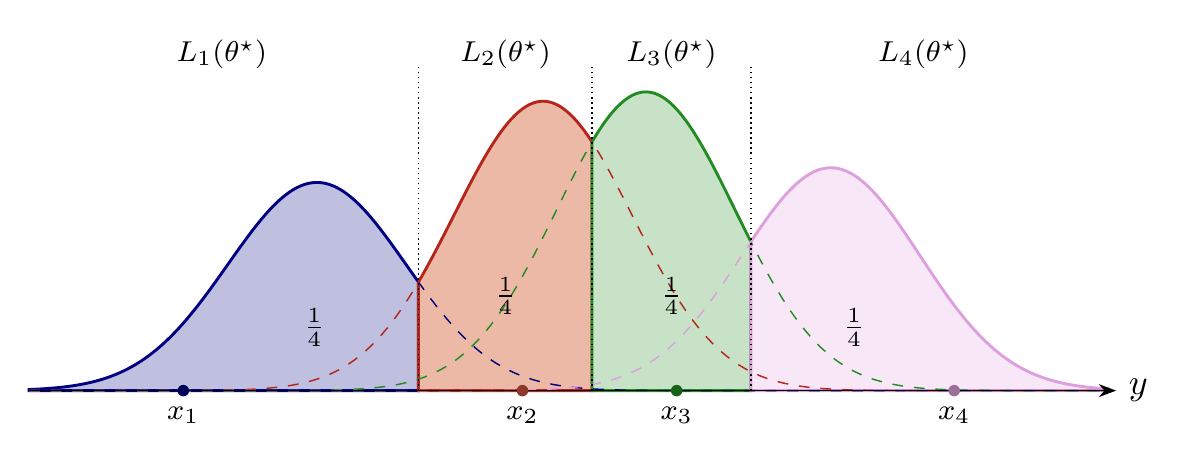
\begin{tikzpicture}[>=Stealth, scale=1.3]
					\begin{axis}[width=\textwidth,height=6cm,axis lines=none,xmin=-3.6,xmax=3.4,ymin=-0.1,ymax=0.33,samples=200,clip=false]
						% tau=1/2, sigma^2=1/3, X=(-2.6,-0.4,0.6,2.4), theta=theta_X^star computed numerically
						% the density of the JKO step: on each cell, the Gaussian of that cell
						\addplot[draw=NavyBlue,thick,fill=NavyBlue!25,domain=-3.6:-1.07485] {0.28638/(sqrt(2*pi)*0.57735)*exp(-(x+1.73333)^2/(2/3))} \closedcycle;
						\addplot[draw=BrickRed,thick,fill=BrickRed!25,domain=-1.07485:0.05080] {0.39808/(sqrt(2*pi)*0.57735)*exp(-(x+0.26667)^2/(2/3))} \closedcycle;
						\addplot[draw=ForestGreen,thick,fill=ForestGreen!25,domain=0.05080:1.08138] {0.41092/(sqrt(2*pi)*0.57735)*exp(-(x-0.4)^2/(2/3))} \closedcycle;
						\addplot[draw=Plum,thick,fill=Plum!25,domain=1.08138:3.4] {0.30657/(sqrt(2*pi)*0.57735)*exp(-(x-1.6)^2/(2/3))} \closedcycle;
						% the four Gaussians A_i n_{X,i}
						\addplot[NavyBlue,dashed,domain=-3.6:3.4] {0.28638/(sqrt(2*pi)*0.57735)*exp(-(x+1.73333)^2/(2/3))};
						\addplot[BrickRed,dashed,domain=-3.6:3.4] {0.39808/(sqrt(2*pi)*0.57735)*exp(-(x+0.26667)^2/(2/3))};
						\addplot[ForestGreen,dashed,domain=-3.6:3.4] {0.41092/(sqrt(2*pi)*0.57735)*exp(-(x-0.4)^2/(2/3))};
						\addplot[Plum,dashed,domain=-3.6:3.4] {0.30657/(sqrt(2*pi)*0.57735)*exp(-(x-1.6)^2/(2/3))};
						% cell boundaries, cell names and masses
						\draw[densely dotted] (axis cs:-1.07485,0)--(axis cs:-1.07485,0.31) (axis cs:0.05080,0)--(axis cs:0.05080,0.31) (axis cs:1.08138,0)--(axis cs:1.08138,0.31);
						\node[font=\footnotesize] at (axis cs:-2.35,0.32) {$L_1(\theta^\star)$};
						\node[font=\footnotesize] at (axis cs:-0.51,0.32) {$L_2(\theta^\star)$};
						\node[font=\footnotesize] at (axis cs:0.566,0.32) {$L_3(\theta^\star)$};
						\node[font=\footnotesize] at (axis cs:2.2,0.32) {$L_4(\theta^\star)$};
						\node[font=\footnotesize] at (axis cs:-1.75,0.06) {$\frac14$};
						\node[font=\footnotesize] at (axis cs:-0.51,0.09) {$\frac14$};
						\node[font=\footnotesize] at (axis cs:0.566,0.09) {$\frac14$};
						\node[font=\footnotesize] at (axis cs:1.75,0.06) {$\frac14$};
						\draw[->] (axis cs:-3.6,0)--(axis cs:3.45,0) node[right] {$y$};
						% points x_i (dots), contracted centres m_i (circles), barycentres b_i (triangles)
						%				\draw[->,gray,shorten >=2pt] (axis cs:-2.6,-0.075) to[out=90,in=-90] (axis cs:-1.73333,-0.004);
						%				\draw[->,gray,shorten >=2pt] (axis cs:-0.4,-0.075) to[out=90,in=-90] (axis cs:-0.26667,-0.004);
						%				\draw[->,gray,shorten >=2pt] (axis cs:0.6,-0.075) to[out=90,in=-90] (axis cs:0.4,-0.004);
						%				\draw[->,gray,shorten >=2pt] (axis cs:2.4,-0.075) to[out=90,in=-90] (axis cs:1.6,-0.004);
						\fill[NavyBlue!70!black] (axis cs:-2.6,0) circle (1.6pt) node[below=1pt,black,font=\footnotesize] {$x_1$}; 
						\fill[BrickRed!70!black] (axis cs:-0.4,0) circle (1.6pt) node[below=1pt,black,font=\footnotesize] {$x_2$}; 
						\fill[ForestGreen!70!black] (axis cs:0.6,0) circle (1.6pt) node[below=1pt,black,font=\footnotesize] {$x_3$}; 
						\fill[Plum!70!black] (axis cs:2.4,0) circle (1.6pt) node[below=1pt,black,font=\footnotesize] {$x_4$}; 
						
%						\draw[NavyBlue!70!black,fill=white] (axis cs:-1.73333,0) circle (1.6pt);
%						\draw[BrickRed!70!black,fill=white] (axis cs:-0.26667,0) circle (1.6pt);
%						\draw[ForestGreen!70!black,fill=white] (axis cs:0.4,0) circle (1.6pt);
%						\draw[Plum!70!black,fill=white] (axis cs:1.6,0) circle (1.6pt);

%						\fill[NavyBlue!70!black] (axis cs:-1.87102,0) ++(0pt,2.6pt) -- ++(-2.3pt,-4pt) -- ++(4.6pt,0pt) -- cycle;
%						\fill[BrickRed!70!black] (axis cs:-0.44428,0) ++(0pt,2.6pt) -- ++(-2.3pt,-4pt) -- ++(4.6pt,0pt) -- cycle;
%						\fill[ForestGreen!70!black] (axis cs:0.52663,0) ++(0pt,2.6pt) -- ++(-2.3pt,-4pt) -- ++(4.6pt,0pt) -- cycle;
%						\fill[Plum!70!black] (axis cs:1.78868,0) ++(0pt,2.6pt) -- ++(-2.3pt,-4pt) -- ++(4.6pt,0pt) -- cycle;
					\end{axis}
%					\node[font=\footnotesize,anchor=north] at ([yshift=+0.2cm]current axis.south) {$\bullet$ points $x_i$};
				\end{tikzpicture}
			}
		\end{center}
	\end{frame}
	
	\begin{frame}[t]{One semi-discrete JKO step 3/3}
		\begin{itemize}
			\item The minimiser $\theta^\star$ is such that
			\begin{equation*}
				\forall i,\qquad \purp{\rho^\star}(L_i(\theta^\star))=\frac1N.
			\end{equation*}
			\vspace{.5\baselineskip}
			\item $\theta^\star\in\mathcal B$ which is explicit
		\end{itemize}
		
		\begin{center}
			\resizebox{0.8\linewidth}{!}{
				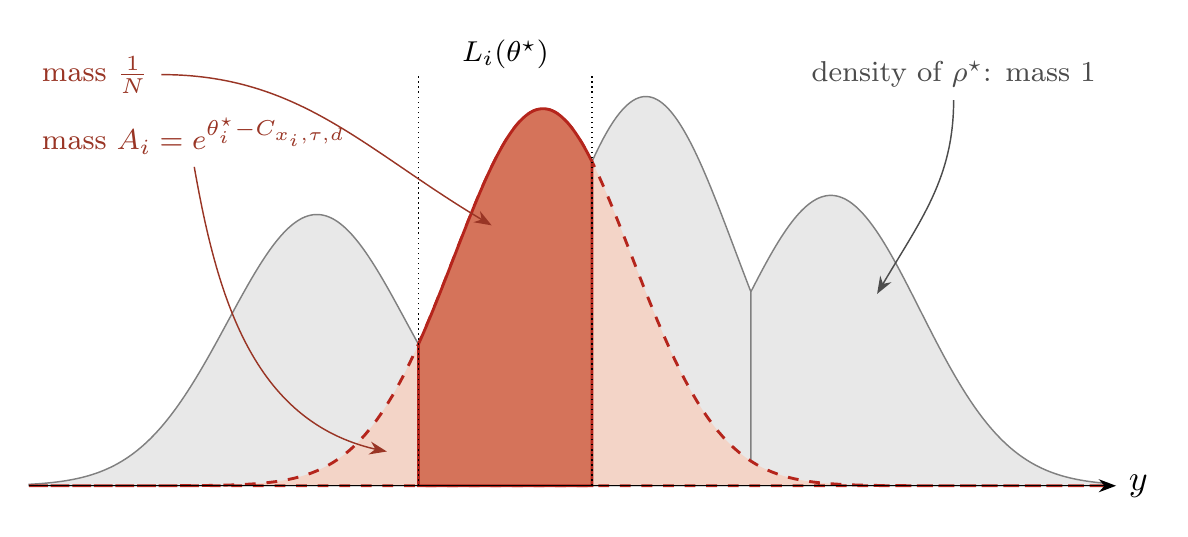
\begin{tikzpicture}[>=Stealth, scale=1.3]
					\begin{axis}[name=ax,width=\textwidth,height=6cm,axis lines=none,xmin=-3.6,xmax=3.4,ymin=0,ymax=0.33,samples=200,clip=false]
						% same cloud as Figure \ref{fig:structure}: tau=1/2, sigma^2=1/3, X=(-2.6,-0.4,0.6,2.4), theta=theta_X^star
						% the density of the JKO step (total mass 1)
						\addplot[draw=gray,fill=gray!18,domain=-3.6:-1.07485] {0.28638/(sqrt(2*pi)*0.57735)*exp(-(x+1.73333)^2/(2/3))} \closedcycle;
						\addplot[draw=gray,fill=gray!18,domain=-1.07485:0.05080] {0.39808/(sqrt(2*pi)*0.57735)*exp(-(x+0.26667)^2/(2/3))} \closedcycle;
						\addplot[draw=gray,fill=gray!18,domain=0.05080:1.08138] {0.41092/(sqrt(2*pi)*0.57735)*exp(-(x-0.4)^2/(2/3))} \closedcycle;
						\addplot[draw=gray,fill=gray!18,domain=1.08138:3.4] {0.30657/(sqrt(2*pi)*0.57735)*exp(-(x-1.6)^2/(2/3))} \closedcycle;
						
						% the whole Gaussian A_i n_{X,i} of the second point (mass A_i)
						\addplot[draw=BrickRed,thick,dashed,fill=BrickRed!15,domain=-3.6:3.4] {0.39808/(sqrt(2*pi)*0.57735)*exp(-(x+0.26667)^2/(2/3))} \closedcycle;
						
						% its part on the Laguerre cell (mass 1/N)
						\addplot[draw=BrickRed,thick,fill=BrickRed!55,domain=-1.07485:0.05080] {0.39808/(sqrt(2*pi)*0.57735)*exp(-(x+0.26667)^2/(2/3))} \closedcycle;
						\draw[densely dotted] (axis cs:-1.07485,0)--(axis cs:-1.07485,0.3) (axis cs:0.05080,0)--(axis cs:0.05080,0.3);
						\node[font=\footnotesize] at (axis cs:-0.51,0.315) {$L_i(\theta^\star)$};
						\draw[->] (axis cs:-3.6,0)--(axis cs:3.45,0) node[right] {$y$};
						
						% labels
						\node[font=\footnotesize,BrickRed!80!black,anchor=west] (cell) at (axis cs:-3.6,0.30) {mass $\frac1N$};
						\draw[BrickRed!80!black,->] (cell.east) to[out=0,in=150] (axis cs:-0.6,0.19);
						\node[font=\footnotesize,BrickRed!80!black,anchor=west] (bump) at (axis cs:-3.6,0.255) {mass $A_i=e^{\theta_i^\star -C_{x_i,\tau,d}}$};
						\draw[BrickRed!80!black,->] (bump.south) to[out=-80,in=170] (axis cs:-1.28,0.025);
						\node[font=\footnotesize,gray!60!black,anchor=east] (dens) at (axis cs:3.4,0.30) {density of $\rho^\star$: mass $1$};
						\draw[gray!60!black,->] (dens.south) to[out=-90,in=60] (axis cs:1.9,0.14);
					\end{axis}
%					\node[anchor=north,align=center] at ([yshift=-0.3cm]ax.south) {$\dfrac1N=\displaystyle\int_{\mathrm{Lag}_i}A_i\pn_{X,i}\;\leq\;\int_{\R^d}A_i\pn_{X,i}=A_i\;\leq\;\int_{\R^d}\max_jA_j\pn_{X,j}=1$,\\[6pt] hence $\theta_{X,i}^\star=a_i+\kappa+\ln{A_i}\in\big[a_i+\kappa-\ln{N},\,a_i+\kappa\big]$.};
				\end{tikzpicture}
			}
		\end{center}
		
	\end{frame}
	
\end{document}